\documentclass[syuuron]{kuee}
\usepackage[dvipdfmx]{graphicx}
\usepackage{kueecite}

\title{評価構造における単語間の関係性可視化に関する研究}
\author{小澤 啓太}
\professor{小山田 耕二 教授}
\course{京都大学大学院 工学研究科}
\department{電気工学専攻}
\date{平成28年2月4日}

%%% 本文
\begin{document}
\maketitle
\tableofcontents


%%%序論
\chapter{序論}
	%%%人々の評価を解明するって大事!
	人々の価値観が多様化している現代社会において,人々がある対象をどのように評価するか、
	何故そのように評価するかという評価の解明が意思決定に必要不可欠となってきた.
	現在、多くの企業にとって市場は自国だけでなく世界全体へと移行しつつあり、
	消費者の好みは年齢や性別、志向性だけでなく国、宗教などによって多様化している. 
	多様化により、商品のターゲット設定も具体的かつ狭まる傾向にあり、より精度の高いマーケティング・リサーチが企業体には必要となっている. 
	精度の高いマーケティング・リサーチには、意思決定の結果がどのような効果をもたらすかエビデンスを用いて議論するエビデンスベースな意思決定が必要である.
	エビデンスベースな意思決定技術の確立は,企業体での意思決定だけでなく国家や個人の意思決定の質の向上という意味でも重要性が高くなってきている.
	
	%%%評価グリッド法って大事
	人々の評価を解明する手法の一つに評価グリッド法という, 半構造化インタビューを用いた定性調査手法がある. 
	評価グリッド法は、環境心理学やマーケティング調査、感性工学といった分野で日本を中心に幅広く利用されており、
	人間が何を知覚して, その知覚からどのような理解をし, どのような価値を見出しているのかというある対象物の評価構造を把握することができる.
	評価構造は「良い-悪い」等,価値判断に寄与している理解の単位 (評価項目) と,評価項目の間に存在する因果関係から構成され, 
	概観を可能にするためネットワーク図として表現されることがある(図~\ref{fig:es1}).
	ネットワーク図で表す場合, 頂点は評価項目を表しており,文章でラベル付けされている(図~\ref{fig:es2}) .また, 評価項目間の因果関係をネットワーク図の枝で表現する. 
	マーケティング分野などでは, この評価構造を分析することで,人間の感性を把握でき, 人間の求める商品の推測につながるので、評価構造の効果的な分析方法に関する要求が高まっている\cite{egm6, egm7}.
	評価構造の分析に関する研究は数多く行われている~\cite{egm8, egm9}. 
	従来の評価構造は、模造紙や付箋などに手書きすることで作成される場合が多く、作成者の大きな負担となっていた. 
	しかし、近年ではE-grid\footnote{http://egrid.jp}のような, 評価グリッド法のインタビューと分析をサポートするWebアプリケーションも開発され, 評価構造作成, 分析の効率化が進んでいる~\cite{egm5, egm6}. 
	
	%%%従来での問題
	E-gridのような評価グリッド法を支援するアプリケーションが増加する中、同時に問題が発生している. 
	それは、評価構造の大規模化に伴う見やすさの低下である. 
	従来の手書きでの作成では大人数の評価構造の統合などが困難であったが、Webアプリケーションなどの登場により容易に行えるようになった. 
	大人数の評価構造が統合されることで、評価項目数が増加し, 指定された領域に評価構造全体を表示するには評価構造を縮小する必要が発生した.  
	縮小された評価構造では評価項目の文字や評価項目間の関係性が見づらく、分析を短時間で行うことが困難になるという問題が発生した. (図~\ref{fig:es3})
	分析する際の着目点として, 評価構造内での頻出語の発見, 頻出語と因果関係を持つ項目の把握があげられる. 
	評価構造内で頻出する単語とは、多くの人が回答した内容である. 
	また、頻出語と隣接する評価項目を知ることで、頻出語が評価されている理由などを知ることができる. 
	このように、頻出する評価項目や頻出語と隣接する評価項目を発見することで消費者の嗜好の傾向を把握することができる. 
	従来の評価構造分析手法では,評価構造を構成する評価項目間の因果関係に着目して因果関係の定量化を行う手法は数多く提案されている~\cite{egm8, egm9}. 
	しかし、評価項目の文章、文章内の単語に着目した評価構造の可視化手法は提案されていない. 
	評価構造の文章や単語に着目することで,頻出語や頻出語と因果関係を持つ項目の発見が容易になるだけでなく、
	似た内容の評価項目の統合にもつながり,評価構造の頂点数が多くなった場合でも分析を行うことができる.
	
	%%%提案手法!手法の説明, 実験の要約
	以上の問題を解決するために本論文は,評価項目内に出現する単語の頻度と,
	評価構造内での単語間の位置関係を反映した評価構造データ向けのテキストベースの可視化手法を提案し, 
	提案手法を用いた評価構造可視化システムの開発を行った. 
	提案システムでは,評価構造内の評価項目の文章を形態素解析し,抽出した単語をWord Cloud技術によって可視化する.
	Word Cloudとは文章中で出現頻度が高い単語を複数選び出し,その頻度に応じた大きさで図示する可視化技術である.
	また, 提案システムではWord Cloud内の単語の配置座標を, 本論文で提案する評価構造内単語の座標計算手法を適用し決定した.
	提案する評価構造内単語の座標計算手法では, はじめに評価構造内での各単語間の位置関係をネットワーク図の最短距離を用いて計算する. 
	この単語の位置関係を多次元尺度構成法により二次元の値に縮小し, この値をWord Cloud内での単語の配置座標とする. 
	しかし, 単語の配置座標決定時は単語間の重複が発生し, 単語間の関係が分かりづらくなる可能性があるので, 
	単語間の位置関係を維持しつつ重複阻止を行った座標をWord Cloud内の単語の配置座標とした. 
	重複阻止では単語間の相対的位置関係の保持を行いつつ, 指定領域の最大活用するためのフォントサイズの最適化も行った. 
	これにより, 単語数に応じて最適なフォントサイズ, 評価構造内での単語の位置関係を保持した読みやすい可視化を達成した. 
	また、提案システムでは指定した単語の関係性を詳細に表示する機能や、評価構造のネットワーク図可視化とWord Cloud可視化を併置し、
	二つの可視化のインタラクティブな操作を可能にすることでより効率的な分析を可能とした. 

	%%%提案手法のもたらす効果
	本論文では, 評価構造のWord Cloud可視化の有効性, Word Cloud内の単語配置方法の有効性を検証するために二種類の比較実験を行った. 
	一つは, 評価構造のWord Cloud可視化の有効性を測るために比較実験を行い, 
	単語数が多い場合の評価構造の頻出単語の発見, 頻出語と因果関係を持つ単語の発見に関してWord Cloud可視化が有効であることを証明した. 
	また, Word Cloud内の単語配置方法の有効性を検証するため, 単語をランダムに配置した場合と提案手法に基づき配置位置を決定した場合とでの比較実験を行った. 
	比較実験により, 頻出単語の発見が容易になり, 単語の座標関係から頻出語と因果関係の強い単語の把握に有効であることが証明された. 
	もう一つの実験は、提案システムの評価として提案システムを用い評価構造の分析を行ってもらい、その後にシステムに関するアンケートを行った. 
	提案システムによって多くの人の共有する評価基準や, その原因の推測に大きく貢献することが期待される. 

	%%%論文構成
	本論文の構成は以下の通りである.
	第1章は,本論文の序論である.第2章は,本論文の関連する研究について述べる. 第3章では,提案手法と使用するデータの説明を行う.
	第4章では,提案システムを用いた評価実験の内容を述べる. 第5章では第4章で行った評価実験の結果を, 第6章では, 考察を行う. 
	最後に, 第7章では本論文の結論と今後の課題について述べる.

		\begin{figure}
			\begin{center}
				\fbox{
				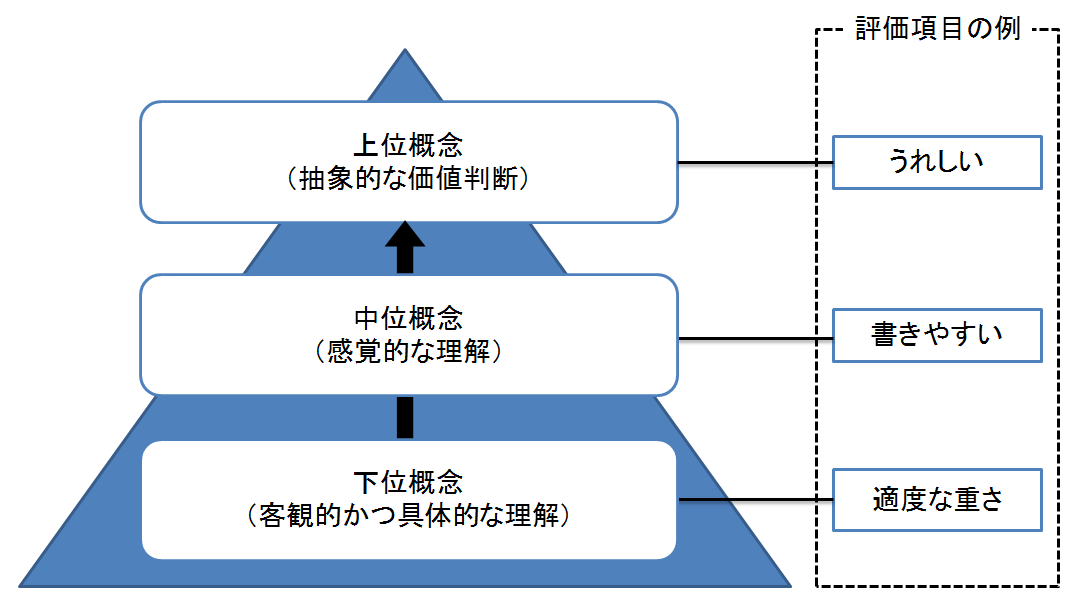
\includegraphics[width=\linewidth]{./png/es1.png}
				}
			\end{center}
			\caption{評価構造の構成}
	  		\label{fig:es1}
		\end{figure}
		\begin{figure}
			\begin{center}
				\fbox{
				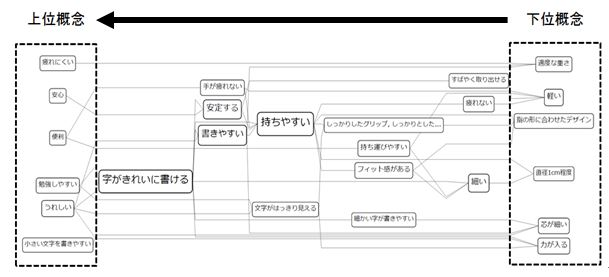
\includegraphics[width=\linewidth]{./png/es2.JPG}
				}
			\end{center}
			\caption{評価構造1}
	  		\label{fig:es2}
		\end{figure}
		\begin{figure}
			\begin{center}
				\fbox{
				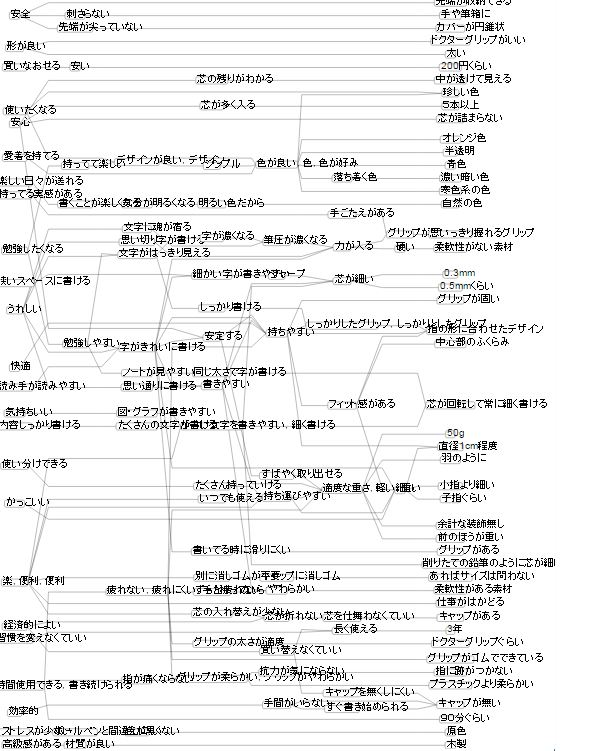
\includegraphics[width=\linewidth]{./png/es3.JPG}
				}
			\end{center}
			\caption{評価構造2}
	  		\label{fig:es3}
		\end{figure}


%======================================================================
%		謝辞
%======================================================================
\begin{acknowledgements}
	ほげ
\end{acknowledgements}



%======================================================================
%		参考文献
%======================================================================
\bibliographystyle{kueethesis}
\bibliography{sotsuron}
\begin{thebibliography}{数字}
	\bibitem{egm1} 奥西智哉, 炊飯米を生地に添加したパンの官能評価. 日本食品科学工学会誌, 56, 424-428, (2009).
	\bibitem{egm2} 入江正和, 豚肉質の評価法. 日本養豚学会誌, 39, 221-254, (2002).
	\bibitem{egm3} 来田宣幸, 赤井聡文. 野球における球速と球速感の関係. 日本認知心理学会発表論文集, 42-42, (2009).
	\bibitem{egm4} 中前光弘, 順位法を用いた視覚評価の信頼性について: 順序尺度の解析と正規化順位法による尺度構成法. 日放技学誌, 56, 725-730, (2000).
	\bibitem{egm5} 大山正, 瀧本誓, 岩澤秀紀. 順位法を用いた視覚評価の信頼性について: 順序尺度の解析と正規化順位法による尺度構成法. 行動計量学, 20, 55-64, (1993).
	\bibitem{egm6} J. Sanui, Visualization of users’requirements: Introduction of Evaluation Grid Method, Proceedings of the 3rd Design and Decision Support System in Architecture and Urban Planning Conference, 365-374, (1996).
	\bibitem{egm7} 讃井純一郎, 乾正雄. レパートリー・グリッド発展手法による住環境評価構造の抽出:認知心理学に基づく住環境評価に関する研究(1). 日本建築学会計画系論文報告集, 367, 15-22, (1986).
	\bibitem{egm8} 尾上洋介, 久木元伸如, 小山田耕二. 可視化情報学会における会員満足度の因果関係分析. 可視化情報学会論文集, 34, 43-51, (2014).
	\bibitem{egm9} 本村陽一, 金出武雄. ヒトの認知・評価構造の定量化モデリングと確率推論. 電子情報通信学会技術研究報告, 104, 25-30, (2005).
	\bibitem{rg1} G. A. Kelly, The Psychology of Personal Constructs, 1 and 2, (1955).
	\bibitem{net1} Y. Onoue, N. Kukimoto, N. Sakamoto, K. Koyamada, Network Coarse-Graining for Evaluation Structures, In Proc. of International Conference on Simulation Technology, 34, 447-450, (2015). 
	\bibitem{kh1} 樋口耕一, テキスト型データの計量的分析. 理論と方法, 19, 101-115, (2004).
	\bibitem{wg1} Riehmann. P, Gruendl. H, Potthast. M, Trenkmann. M, Stein. B, Froehlich. B, WORDGRAPH: Keyword-in-Context Visualization for NETSPEAK's Wildcard Search. Visualization and Computer Graphics, IEEE Transactions on 18.9, 1411-1423, (2012).
	\bibitem{rwc1} Strobelt. H, Spicker. M, Stoffel. A, Keim. D, Deussen. O, Rolled‐out Wordles: A Heuristic Method for Overlap Removal of 2D Data Representatives, Computer Graphics Forum, 31, 1135-1144, (2012).
	\bibitem{fta1} Huang. X, Lai. W, Force-transfer: a new approach to removing overlapping nodes in graph layout, Proceedings of the 26th Australasian computer science conference, 16, 349-358, (2003).
	\bibitem{or1} Gomez-Nieto. E, San Roman. F, Pagliosa. P, Casaca. W, Helou. E. S, Oliveira. M. C. F, Nonato. L. G, Similarity Preserving Snippet-Based Visualization of Web Search Results, Visualization and Computer Graphics, IEEE Transactions on, 20, 457-470, (2014).
	\bibitem{or2} Gomez-Nieto. E, Casaca. W, Motta. D, Hartmann. I, Taubin. G, Nonato. L, Dealing with Multiple Requirements in Geometric Arrangements, Visualization and Computer Graphics, IEEE Transactions on, 1, (2015).
	\bibitem{mcb1} T. Kuo, K. Yamamoto, Y. Matsumoto, Applying Conditional Random Fields to Japanese Morphological Analysis, Proceedings of the 2004 conference on empirical methods in natural language processing, 230-237, (2004).
	\bibitem{hak1} 尾上洋介, 評価構造のビジュアル分析に関する研究,博士論文, 2016.
\end{thebibliography}

%======================================================================
%		付録
%======================================================================
\appendix


\end{document}
% Local Variables:
% fill-column: 70
% End:
